\documentclass{esg8012exam}
\begin{preamble}
  \usepackage{amsmath}
  \usepackage{amssymb}
  \usepackage{enumerate}
  \usepackage{graphicx}
  \usepackage{hyperref}
  \usepackage{siunitx}
  \providecommand{\uvec}[1]{{\hat{\bf{#1}}}}
  \usepackage{pgf,tikz}
  \usetikzlibrary{arrows}
  \usepackage{subfigure}
  %\usepackage{wrapfig} 
  \newcommand{\subfigureautorefname}{\figureautorefname}
  \makeatletter
  \newcommand{\interitemtext}[1]{%
    \begin{list}{}
     {\itemindent=0mm\labelsep=0mm
     \labelwidth=0mm\leftmargin=0mm
     \addtolength{\leftmargin}{-\@totalleftmargin}}
      \item #1
    \end{list}
  }
  \makeatother
  \renewcommand{\d}{\,d}
  \providecommand{\norm}[1]{\lVert#1\rVert}
\end{preamble}

\classname{Physics 8.012}
\semester{Fall 2010}
\examnumber{1}

\begin{document}

\begin{problem}{(30 Points)}
  A car is driving through a green light at $t = 0$ located at $x = 0$ with an initial speed $v_{c, 0} = \SI{12}{\meter\per\second}$.  The acceleration of the car as a function of time is given by
  $$a_c = \begin{cases}
            0 & \text{if }0 < t < t_1 = \SI{1}{\second} \\
            -(\SI{6}{\meter\per\second\cubed})(t - t_1) & \text{if }\SI{1}{\second} < t < t_2
          \end{cases}
  .$$
  A bicycle rider is riding at a constant speed of $v_{b,0}$ and at $t = 0$ is \SI{17}{\meter} behind the car.  The bicyclist reaches the car when the car just comes to rest at time $t_2$.

  \begin{enumerate}[(a)]
    \item Find the time $t_2$ that the car has just come to rest.
    \item Find the speed of the bicycle.
  \end{enumerate}
\end{problem}
\begin{solution}
  \subsubsection{Getting started}
    We choose a coordinate system with the car and bicycle moving in the positive $x$-direction, and label the position of the car as a function of time by $x_c(t)$ and the position of the bicycle as a function of time by $x_b(t)$.  We choose the origin such that at $t = 0$, the car is at the origin $x_c(0) = 0$ and the bicycle is $x_b(0) = -\SI{17}{\meter}$
.  The initial $x$-component of the velocity of the car is $v_{x,c}(0) \equiv v_{c,x,0} = \SI{12}{\meter\per\second}$.  The initial $x$-component of the velocity of the bicycle is denoted by $v_{x,b}(0) \equiv v_{b,x,0}$ and is the quantity we are trying to find.
  \subsubsection{Strategy}
    We first identify that the car has two stages of motion, and that at some instant $t_2$ during the second stage of motion, the bicycle and car intersect when $x$-component of the velocity of the car is zero. We can express these two conditions as
    \begin{align}
      x_c(t_2) & = x_b(t_2) \label{eq:car_bike_same_final_pos}\\
      v_{x,c}(t_2) & = 0 \label{eq:car_final_rest}
    \end{align}
    Because we are given the piecewise function for the $x$-component of the acceleration of the car for the two stages of motion, the initial conditions, and the length of the first stage of motion, we can integrate the $x$-component of the acceleration to find the $x$-component of the velocity of the car.  We can find $t_2$ by solving \autoref{eq:car_final_rest}.  We can integrate the $x$-component of the velocity of the car to find the position of the car $x_c(t)$.  We are also told that the car is moving at a constant speed so we can easily find the position function $x_b(t)$ which will be a depend on the unknown initial speed $v_{x,b}(0) \equiv v_{b,x,0}$.  We can then use \autoref{eq:car_bike_same_final_pos} to solve for $v_{x,b}(0) \equiv v_{b,x,0}$.
  \subsubsection{Carrying out the plan}
    For the first stage of motion of the car during the interval $0 < t < t_1 = \SI{1}{\second}$, the car is not accelerating so the speed is constant and hence
    $$v_c(t) = v_{c,0},\qquad 0 < t < t_1 = \SI{1}{\second}.$$
    For the second stage of motion
    $$v_c(t) - v_c(t_1) = \int_{t_1}^t -(\SI{6}{\meter\per\second\cubed})(t - t_1)\,dt,\qquad \SI{1}{\second} < t < t_2$$
    Keep in mind that the end conditions of the first stage of motion are the initial conditions for the second stage of motion so $v_c(t_1) = v_{c,0} = \SI{12}{\meter\per\second}$. Thus after integrating we get
    $$v_c(t) = \SI{12}{\meter\per\second} - \left.(\SI{3}{\meter\per\second\cubed})(t - t_1)^2\right|_{t_1}^t,\qquad \SI{1}{\second} < t < t_2$$
    Now substitute the endpoint so the integral to finally yield
    \begin{equation}
      v_c(t) = \SI{12}{\meter\per\second} - (\SI{3}{\meter\per\second\cubed})(t - t_1)^2,\qquad \SI{1}{\second} < t < t_2 \label{eq:car_second_velocity}
    \end{equation}
    Thus the $x$-component of the velocity of the car for the entire motion is given by
    \begin{equation}
      v_c(t) = \begin{cases}
                v_{c,0} = \SI{12}{\meter\per\second} & \text{if }0 < t < t_1 = \SI{1}{\second} \\
                \SI{12}{\meter\per\second} - (\SI{3}{\meter\per\second\cubed})\left(t - (\SI{1}{\second})\right)^2 & \text{if }\SI{1}{\second} < t < t_2
               \end{cases}
    \end{equation}
    We can use now \autoref{eq:car_final_rest} to find the time $t_2$ that the car came to rest,
    $$0 = v_c(t_2) = \SI{12}{\meter\per\second} - (\SI{3}{\meter\per\second\cubed})\left(t_2 - (\SI{1}{\second})\right)^2.$$
    Solving for $t_2$ (using the positive square root)
    \begin{equation}
      t_2 = \SI{1}{\second} + \sqrt{\SI{12}{\meter\per\second} / (\SI{3}{\meter\per\second\cubed})} = \SI{3}{\second}
    \end{equation}
    \textsc{Note}: We have two solutions: $t_2 - t_1 = \SI{2}{\second}$ or $t_2 - t_1 = -\SI{2}{\second}$.  The second solution $t_2 = t_1 - \SI{2}{\second} = \SI{1}{\second} - \SI{2}{\second} = -\SI{1}{\second}$ does not apply to our time interval.
    
    For this one dimensional motion the change in position of the car as a function of time for the first stage of motion is given by
    $$x_c(t) - x_c(0) = \int_0^t v_{x,c,0}\,dt = v_{x,c,0}t = (\SI{12}{\meter\per\second})t,\qquad 0 < t < t_1 = \SI{1}{\second}$$
    Because the car started at the origin, the position at the end of the interval is given by
    $$x_c(t_1) = (\SI{12}{\meter\per\second})t_1 = (\SI{12}{\meter\per\second})(\SI{1}{\second}) = \SI{12}{\meter}.$$
    For the second stage of motion, the change in position is given by the integral of the $x$-component of the velocity for stage two (\autoref{eq:car_second_velocity}),
    $$x_c(t) - x_c(t_1) = \int_{t_1}^t \left( \SI{12}{\meter\per\second} - (\SI{3}{\meter\per\second\cubed})(t - t_1)^2\right)\,dt,\qquad \SI{1}{\second} < t < t_2$$
    Upon integration we have
    $$x_c(t) = x_c(t_1) + \left.\left( (\SI{12}{\meter\per\second})(t - t_1) - (\SI{1}{\meter\per\second\cubed})(t - t_1)^3\right)\right|_{t_1}^t,\qquad \SI{1}{\second} < t < t_2$$
    So after substituting $x_c(t_1) = \SI{12}{\meter}$ and substituting in the endpoints of the integration interval we have that for the second stage of motion
    \begin{equation}
      x_c(t) = \SI{12}{\meter} + (\SI{12}{\meter\per\second})(t - t_1) - (\SI{1}{\meter\per\second\cubed})(t - t_1)^3,\qquad \SI{1}{\second} < t < t_2 \label{eq:car_pos_second}
    \end{equation}
    Combining our results, the position of the car as function of time is given by
    \begin{equation}
      x_c(t) = \begin{cases}
                (\SI{12}{\meter\per\second})t & \text{if }0 < t < t_1 = \SI{1}{\second} \\
                \SI{12}{\meter} + (\SI{12}{\meter\per\second})(t - t_1) - (\SI{1}{\meter\per\second\cubed})(t - t_1)^3 & \text{if }\SI{1}{\second} < t < t_2
               \end{cases}
    \end{equation}
    We can find the position of the car when the $x$-component of velocity of the car is zero, by setting $t = t_2 = \SI{3}{\second}$ in \autoref{eq:car_pos_second} and noting that $t_2 - t_1 = \SI{3}{\second} - \SI{1}{\second} = \SI{2}{\second}$: 
    \begin{equation}
      x_c(t_2) = \SI{12}{\meter} + (\SI{12}{\meter\per\second})(\SI{2}{\second}) - (\SI{1}{\meter\per\second\cubed})(\SI{2}{\second})^3 = \SI{28}{\meter} \label{eq:car_final_position}
    \end{equation}
    \paragraph{Speed of the bicycle}
      Since the bicycle is traveling at a constant speed with an initial position $x_{b,0} = -\SI{17}{\meter}$, the position of the bicycle as a function of time is given by
      $$x_b(t) = -\SI{17}{\meter} + v_{b,x,0}t.$$
      At $t = t_f$,
      \begin{equation}
        x_b(t_f) = -\SI{17}{\meter} + v_{b,x,0}t_f \label{eq:bicycle_final_position}
      \end{equation}
      Because the bicycle and car intersect at $t = t_f$, we can now use \autoref{eq:car_bike_same_final_pos}, \autoref{eq:bicycle_final_position}, and \autoref{eq:car_final_position} to find the initial speed of the bicycle
      $$-\SI{17}{\meter} + v_b(\SI{3}{\second}) = \SI{28}{\meter}.$$
      So the speed of the bicycle is
      $$v_b = \frac{\SI{28}{\meter} + \SI{17}{\meter}}{\SI{3}{\second}} = \SI{15}{\meter\per\second}.$$
\end{solution}





\begin{problem}{(30 Points)}
  Two blocks with masses $m_1$ and $m_2$ such that $m_1 \ll m_2$ are connected by a massless inextensible string and a massless pulley as shown in the figure below.  The pulley is rigidly connected to the top of a wedge with angle $\theta$.  The coefficient of friction between the blocks is $\mu$.  The surface between the lower block and the wedge is frictionless.  What are the magnitudes of the acceleration of the two blocks?
  \begin{center}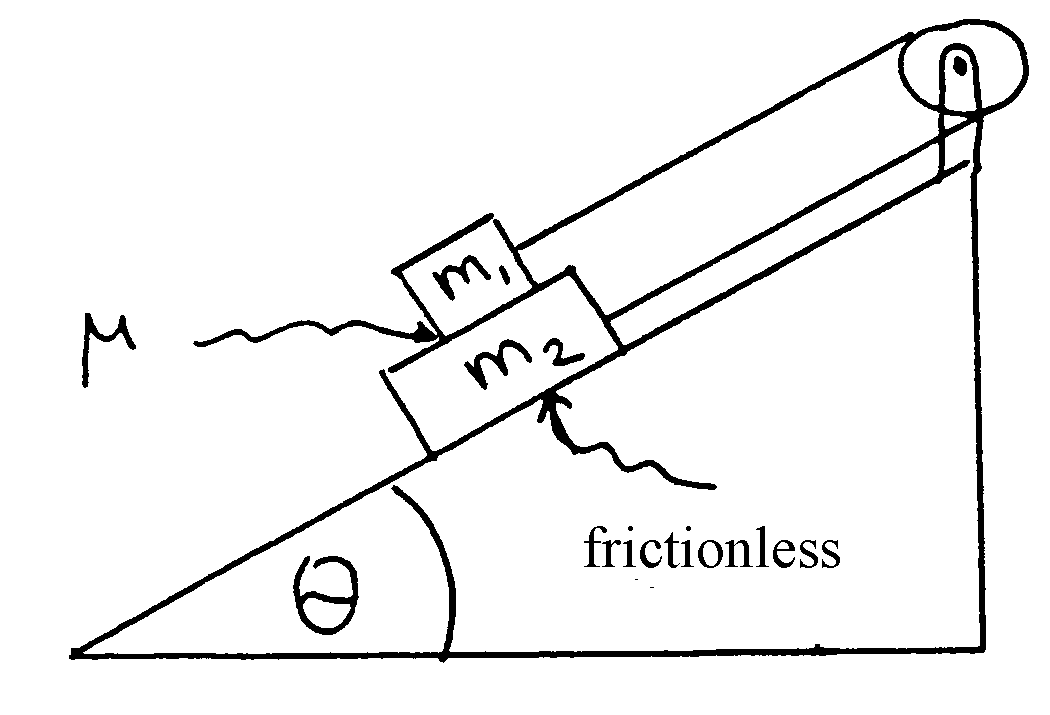
\includegraphics[width=0.33\textwidth]{exam1_p2_1}\end{center}
\end{problem}
\begin{solution}
  We shall apply Newton's Second Law to each block. Since the blocks are constrained by the rope, the accelerations of the blocks must be related. We should be able to then simultaneously solve the equations of motion for each block to find the magnitude of the acceleration. We begin by choosing a coordinate system shown in \autoref{fig:2_coordinate_system}.
  \begin{figure}[h!]%
    \begin{center}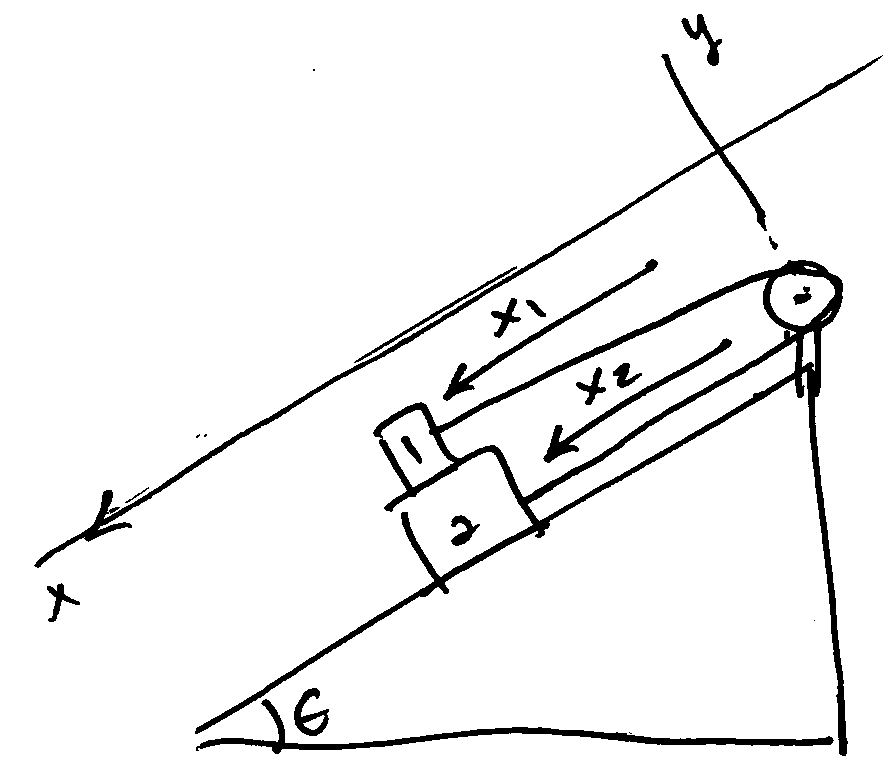
\includegraphics[width=0.3\textwidth]{exam1_s2_1}\end{center}%
    \caption{Coordinate System}
    \label{fig:2_coordinate_system}%
  \end{figure}
  We then draw free body force diagrams for each object. We show these in \autoref{fig:2_free_body_1} and \autoref{fig:2_free_body_2}. \par
  \begin{figure}[h!]
    \begin{center}
      \subfigure[Object 1]{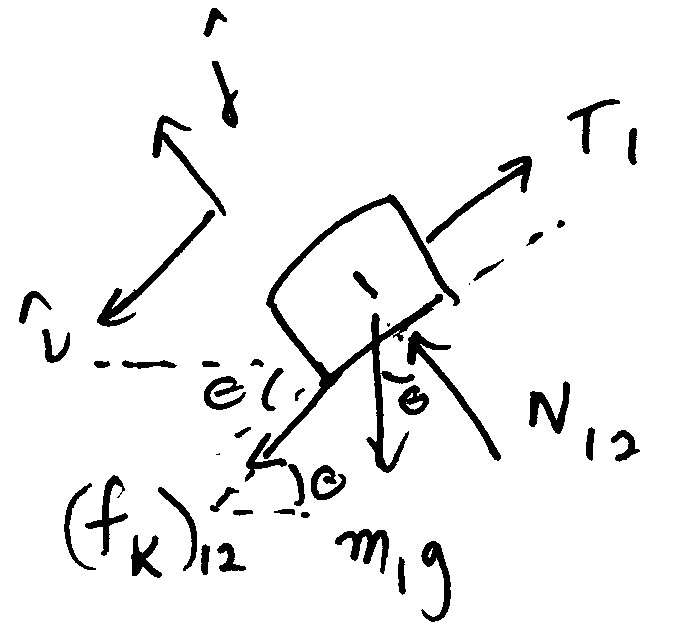
\includegraphics[width=0.33\textwidth]{exam1_s2_2} \label{fig:2_free_body_1}}
      \subfigure[Object 2]{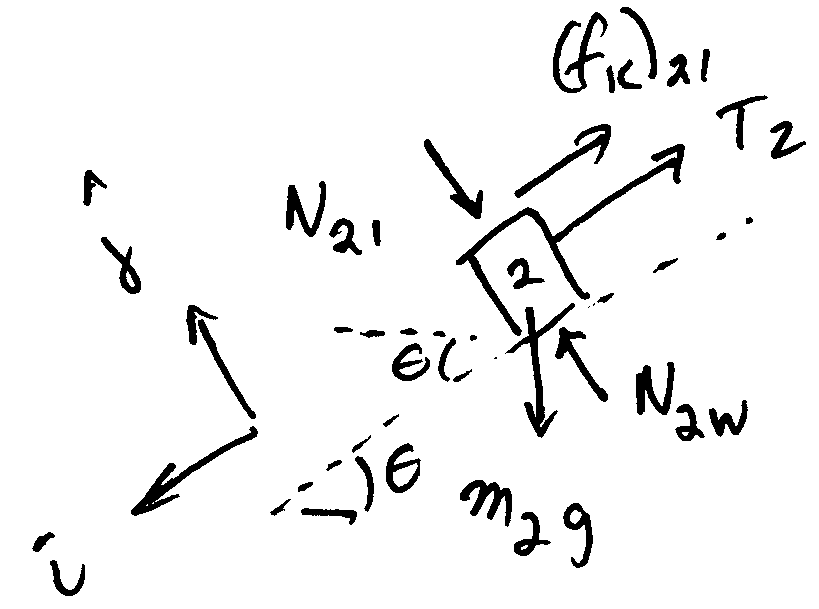
\includegraphics[width=0.33\textwidth]{exam1_s2_3} \label{fig:2_free_body_2}}
    \end{center}
    \caption{Free Body Diagrams}
  \end{figure}
  Newton's Second law on object 1 becomes
  \begin{align}
    \uvec j\!: & N_{12} - m_1 g \cos\theta = 0 \label{eq:2_j_object_1} \\
    \uvec i\!: & m_1 g \sin\theta + (f_k)_{12} - T_1 = m_1 a_{x,1}. \label{eq:2_i_object_1}
  \end{align}
  Newton's Second law on object 2 becomes
  \begin{align}
    \uvec j\!: & N_{2W} - N_{21} - m_2 g \cos\theta = 0 \label{eq:2_j_object_2} \\
    \uvec i\!: & m_2 g \sin\theta + (f_k)_{21} - T_2 = m_2 a_{x,2}. \label{eq:2_i_object_2}
  \end{align}
  We can use \autoref{eq:2_j_object_1} to solve for the normal force between the surfaces,
  \begin{equation}
    N_{12} = m_1 g \cos\theta. \label{eq:2_normal_force}
  \end{equation}
  We note that because we assumed that the string is massless and inextensible the tension in the string is uniform, so
  \begin{equation}
    T \equiv T_1 = T_2. \label{eq:2_tension}
  \end{equation}
  We note that the contact force between the blocks form an action-reaction pair.  When we decompose this force into its tangent (kinetic friction) and perpendicular (normal force) components, we have that
  \begin{equation}
    f_k \equiv (f_k)_{12} = (f_k)_{21}. \label{eq:2_friction}
  \end{equation}
  From \autoref{eq:2_normal_force}
  \begin{equation}
    N \equiv N_{12} = N_{21} = m_1 g \cos\theta. \label{eq:2_normal_gravity}
  \end{equation}
  Also we model the kinetic friction by the force law
  \begin{equation}
    f_k = \mu N = \mu m_1 g \cos\theta. \label{eq:2_friction_gravity}
  \end{equation}
  Finally we note that the $x$-components of the accelerations of the two objects are related by
  \begin{equation}
    a \equiv a_{x,2} = -a_{x,1}. \label{eq:2_acceleration}
  \end{equation}
  Note that $a$ is also the magnitude of the acceleration of the blocks because we expect that $a \equiv a_{x, 2} > 0$. Thus using \autoref{eq:2_tension}, \autoref{eq:2_friction}, \autoref{eq:2_normal_gravity}, and \autoref{eq:2_friction_gravity} we can rewrite \autoref{eq:2_i_object_1} as
  \begin{equation}
    m_1 g \sin\theta + \mu m_1 g \cos\theta - T = -m_1 a \label{eq:2_rewrite_i_object_1}
  \end{equation}
  and \autoref{eq:2_i_object_2} as
  \begin{equation}
    m_2 g \sin\theta - \mu m_1 g \cos\theta - T = m_2 a. \label{eq:2_rewrite_i_object_2}
  \end{equation}
  We have two unknowns $T$ and $a$, and two independent equations so we can algebraically solve for the magnitude of the acceleration of the blocks.
  
  We subtract \autoref{eq:2_rewrite_i_object_2} from \autoref{eq:2_rewrite_i_object_1} yielding
  \begin{equation}
    (m_1 g \sin\theta + \mu m_1 g \cos\theta - T) - (m_2 g \sin\theta - \mu m_1 g \cos\theta - T) = -m_1 a - m_2 a.
  \end{equation}
  This simplifies to
  \begin{equation}
    (m_1 - m_2) g \sin\theta + 2\mu m_1 g \cos\theta = -(m_1 + m_2) a.
  \end{equation}
  We can solve this for the magnitude of the acceleration of the blocks:
  \begin{equation}
    a = \frac{(m_2 - m_1) g \sin\theta - 2\mu m_1 g \cos\theta}{m_1 + m_2}.
  \end{equation}
  
  \textsc{Remark}: If the constraint condition \autoref{eq:2_acceleration} is not immediately obvious, consider that the length of the string is given by
  \begin{equation}
    l = x_1 + x_2 + \pi R,\label{eq:2_length}
  \end{equation}
  where $R$ is the radius of the pulley.  Since the length of the string is constant we can differentiate \autoref{eq:2_length} twice with respect to time to find that
  \begin{equation}
    \frac{d^2l}{dt^2} = \frac{d^2x_2}{dt^2} + \frac{d^2x_2}{dt^2} + \pi \frac{d^2R}{dt^2}. \label{eq:2_length_derivative}
  \end{equation}
  Since $R$ and $l$ are constants,
  \begin{equation}
    \frac{d^2l}{dt^2} = 0\quad\text{and}\quad\pi\frac{d^2R}{dt^2} = 0.
  \end{equation}
  Then \autoref{eq:2_length_derivative} becomes
  \begin{equation}
    0 = \frac{d^2x_2}{dt^2} + \frac{d^2x_2}{dt^2} = a_{x, 1} + a_{x, 2},
  \end{equation}
  thus justifying \autoref{eq:2_acceleration}.
\end{solution}



\clearpage

\begin{problem}{(30 Points)}
  A U-control airplane of mass $M$ is attached by a wire of length $L$ and negligible mass to the ``pilot'' who controls the ``lift'' provided by the wing, the force that is normal to the plane of the wings keeping the plane aloft and hence in a direction perpendicular to the wire.  The plane's engine keeps it moving at constant speed $v$.  The wire and the wings of the plane make an angle $\theta$ with the ground.  The gravitational acceleration is $g$.  Express your answers to the following questions in terms of $M$, $g$, $L$, $v$, and $\theta$ as needed.
  \begin{enumerate}[(a)]
    \item Find the tension $T$ in the wire when the plane is flown overhead in a circle.
    \item Find a condition that the speed of the plane must satisfy such that, for all values of $\theta$, the tension in the string is not zero. (\textsc{Note}: Your condition should \emph{not} depend on $\theta$.)
    \item Find the magnitude of the ``lift'', the force that is normal to the plane of the wings keeping the plane aloft.
    \item Based on your result form part (c), is $\theta = \pi / 2$ possible?
  \end{enumerate}
  \begin{center}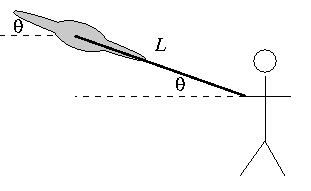
\includegraphics[width=0.4\textwidth]{exam1_p3_1}\end{center}
\end{problem}
\begin{solution}
  \begin{enumerate}[(a)]
    \item Choose polar coordinates. The free body force diagram is shown below. 
      \begin{center}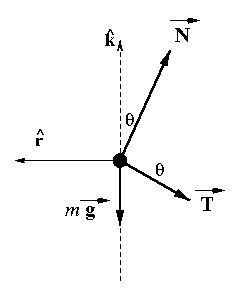
\includegraphics[width=0.3\textwidth]{exam1_s3_1}\end{center}
      Then Newton's Second Law in the vertical direction becomes
      \begin{equation}
        N\cos\theta - T\sin\theta - M g = 0. \label{eq:3_newton_vertical}
      \end{equation}
      Newton's Second Law in the radial direction becomes
      \begin{equation}
        - N \sin\theta - T \cos\theta = -\frac{M v^2}{L \cos\theta} \label{eq:3_newton_radial}
      \end{equation}
      where $r = L\cos\theta$ is the radius of the circular orbit of the plane. 
      \par
      Multiplying \autoref{eq:3_newton_radial} by $\cos\theta$ yields
      \begin{equation}
        N\sin\theta\cos\theta + T \cos^2 \theta = \frac{M v^2}{L}. \label{eq:3_radial_times_cos}
      \end{equation}
      Multiplying \autoref{eq:3_newton_vertical} by $\sin\theta$ yields
      \begin{equation}
        N\cos\theta\sin\theta + T \sin^2 \theta = M g\sin\theta. \label{eq:3_vertical_times_sin}
      \end{equation}
      Subtract \autoref{eq:3_vertical_times_sin} from \autoref{eq:3_radial_times_cos} and use the identity $\cos^2\theta + \sin^2\theta = 1$ to get an expression for the tension:
      \begin{equation}
        T = M\left(\frac{v^2}{L} - g \sin\theta\right). \label{eq:3_tension}
      \end{equation}
    \item Then tension in the wire is zero when 
      \begin{equation}
        \frac{v^2}{g L} = \sin\theta
      \end{equation}
      Since $\sin\theta \le 1$, if $v^2 > gL$ then the tension is never zero for any possible angle $\theta$.
    \item Multiplying \autoref{eq:3_newton_vertical} by $\cos\theta$ yields
      \begin{equation}
        N \cos^2\theta - T\cos\theta\sin\theta - M g \cos\theta = 0. \label{eq:3_vertical_times_cos}
      \end{equation}
      Multiplying \autoref{eq:3_newton_radial} by $-\sin\theta$ yields
      \begin{equation}
        N \sin^2\theta + T\sin\theta\cos\theta = \frac{M v^2}{L}\tan\theta. \label{eq:3_radial_times_-sin}
      \end{equation}
      Add \autoref{eq:3_vertical_times_cos} and \autoref{eq:3_radial_times_-sin}, use the identity $\cos^2\theta + \sin^2\theta = 1$, and do some rearranging to get an expression for the magnitude of the lift force:
      \begin{equation}
        N = M g \cos\theta + \frac{M v^2}{L} \tan\theta
      \end{equation}
    \item As $\theta \to \pi / 2$, $\tan\theta \to \infty$, and hence $N \to \infty$ which is not possible.
  \end{enumerate}
\end{solution}




%\begin{wrapfigure}{r}{0.2\textwidth}
  %\begin{center}
    %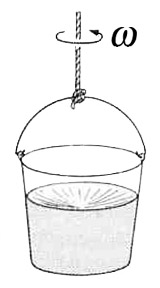
\includegraphics[width=0.18\textwidth]{exam1_p4_1}
  %\end{center}
%\end{wrapfigure}
\begin{problem}{(10 Points)}
  A bucket of water spins with angular speed $\omega$.  What shape does the water's surface assume.  That is, find an equation for the surface of the water.  Clearly show your coordinate system, free body diagram, and all relevant work.
  \begin{center}
    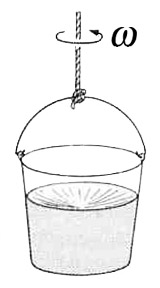
\includegraphics[width=0.18\textwidth]{exam1_p4_1}
  \end{center}
\end{problem}
\begin{solution}
  \subsubsection{Solution with perpendicular normal force}
    Since the pressure on a small bit of water is uniform on all sides, the normal force is perpendicular to the tangent line.  (Alternatively, note that, unlike solids, liquids cannot exert surface tangential forces in equilibrium.)  Then the force diagram is
    \begin{center}
      \begin{tikzpicture}[line cap=round,line join=round,>=triangle 45,x=1.5cm,y=1.5cm]
      \clip(-0.5,-0.5) rectangle (6,4);
      \draw [samples=50,rotate around={0:(0,0)},domain=-0.5:6,xshift=0,yshift=0] plot (\x,\x^2/19.6133);
      \draw[->,color=black] (-0.5,0) -- (6,0);
      \draw[color=black] (5.75,0.04) node [anchor=south west] {$r$};
      \draw[->,color=black] (0,-0.5) -- (0,4);
      \draw[color=black] (0.05,3.81) node [anchor=west] {$z$};
      \draw [shift={(3.82,0.74)}] (0,0) -- (90:0.31) arc (90:111.29:0.31) -- cycle;
      \draw [shift={(3.82,0.74)}] (0,0) -- (0:0.31) arc (0:21.29:0.31) -- cycle;
      \draw [line width=0.4pt] (3.82,-1.26)-- (3.82,2.74);
      \draw [->,line width=1pt] (3.82,0.74) -- (3.54,1.48);
      \draw [->,line width=1pt] (3.82,0.74) -- (3.82,0.01);
      \draw [line width=0.4pt] (1.82,0.74)-- (5.82,0.74);
      \draw [line width=0.4pt] (3.1,2.61)-- (4.55,-1.12);
      \draw [line width=0.4pt] (5.69,1.47)-- (1.96,0.02);
      \draw [line width=0.4pt,dash pattern=on 2pt off 2pt] (3.82,0.74)-- (0,0.74);
      \draw (0,0.74)-- (0,0);
      \draw [->,line width=1pt] (0.74,2.59) -- (0.74,3.59);
      \draw [->,line width=1pt] (0.74,2.59) -- (1.74,2.59);
      \draw[color=black] (3.42,1.35) node {$N$};
      \draw[color=black] (3.58,0.18) node {$mg$};
      \draw[color=black] (3.75,1.2) node {$\theta$};
      \draw[color=black] (4.37,0.86) node {$\theta$};
      \draw[color=black] (1.92,0.98) node {$r$};
      \draw[color=black] (-0.13,0.46) node {$z$};
      \draw[color=black] (0.98,3.58) node {$\hat k$};
      \draw[color=black] (1.82,2.76) node {$\hat r$};
      \end{tikzpicture}
    \end{center}
    Newton's Second Law gives us
    \begin{align}
      \uvec r\!: & -N\sin\theta = -m r \omega^2 \label{eq:4_r} \\
      \uvec k\!: & N \cos\theta = m g \label{eq:4_k}
    \end{align}
    Dividing \autoref{eq:4_r} by \autoref{eq:4_k} and negating both sides,
    \begin{equation}
      \tan\theta = \frac{r\omega^2}{g}.
    \end{equation}
    We also have that $\tan\theta$ is the slope of the tangent line:
    $$\frac{r\omega^2}{g} = \tan\theta = \frac{dz}{dr}.$$
    Manipulating the differentials and integrating both sides,
    $$z = \int_0^z\,dz = \int_0^r \frac{r\omega^2}{g}\,dr = \frac{1}{2}\frac{\omega^2}{g}r^2 = \frac{\omega^2 r^2}{2g}.$$
  \subsubsection{Solution by pressure}
    A partial diagram of a two-dimensional slice is
    \begin{center}
\begin{tikzpicture}[line cap=round,line join=round,>=triangle 45,x=2.0cm,y=2.0cm]
\draw[->,color=black] (-0.5,0) -- (6,0);
\foreach \x in {,1,2,3,4,5}
\draw[shift={(\x,0)},color=black] (0pt,-2pt);
\draw[color=black] (5.83,0.04) node [anchor=south west] {$r$};
\draw[->,color=black] (0,-0.5) -- (0,4);
\foreach \y in {,1,2,3}
\draw[shift={(0,\y)},color=black] (2pt,0pt) -- (-2pt,0pt);
\draw[color=black] (0.05,3.8) node [anchor=west] {$z$};
\clip(-0.5,-0.5) rectangle (6,4);
\draw [shift={(3.77,0.7)},fill=black,fill opacity=0.1] (0,0) -- (0:0.33) arc (0:24.38:0.33) -- cycle;
\draw [samples=50,rotate around={0:(0,0)},xshift=0cm,yshift=0cm] plot (\x,\x^2/2/9.80665);
\draw [line width=0.4pt] (6.27,1.83)-- (2.62,0.18);
\draw [line width=0.4pt,dash pattern=on 2pt off 2pt] (4.45,1.01)-- (0,1.01);
\draw (0,1.01)-- (0,0);
\draw [->,line width=1.6pt] (0.74,2.59) -- (0.74,3.59);
\draw [->,line width=1.6pt] (0.74,2.59) -- (1.74,2.59);
\draw (5.12,1.31)-- (5.12,0.7);
\draw (5.12,0.7)-- (3.77,0.7);
\draw [line width=0.4pt] (5.12,3.01)-- (5.12,-0.99);
\draw [line width=0.4pt] (6.45,0.7)-- (2.45,0.7);
\draw [->,line width=1.2pt] (4.78,0.85) -- (4.78,0.12);
\draw[color=black] (2.24,1.26) node {$r$};
\draw[color=black] (-0.12,0.59) node {$z$};
\draw[color=black] (1.06,3.61) node {$\hat k$};
\draw[color=black] (1.93,2.77) node {$\hat r$};
\draw[color=black] (4.38,0.81) node {$\theta$};
\draw[color=black] (5.17,1.09) node {$\Delta z$};
\draw[color=black] (4.63,0.63) node {$\Delta r$};
\draw[color=black] (4.74,0.15) node {$\Delta mg$};
\end{tikzpicture}
    \end{center}
    Looking at the forces acting on the small water element,
    \begin{center}
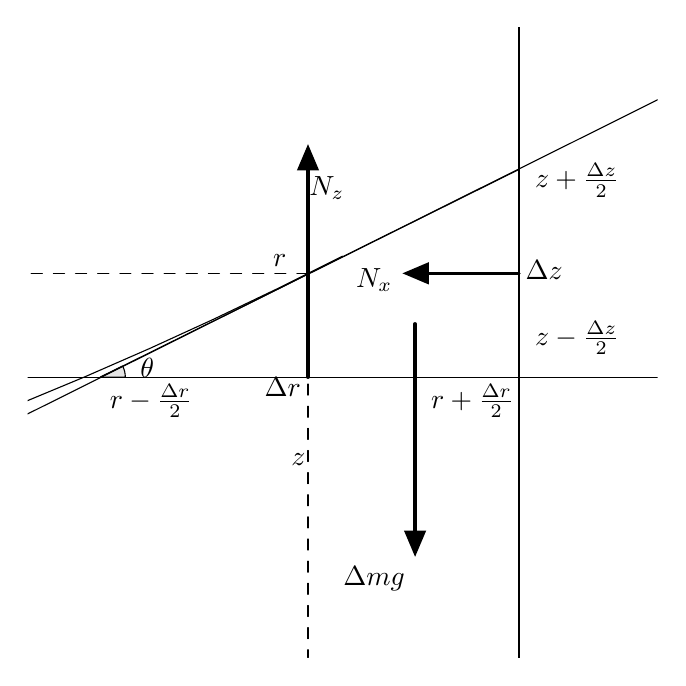
\begin{tikzpicture}[line cap=round,line join=round,>=triangle 45,x=4.0cm,y=4.0cm]
\clip(4,0) rectangle (6,2);
\draw [shift={(4.23,0.89)},fill=black,fill opacity=0.1] (0,0) -- (0:0.08) arc (0:26.53:0.08) -- cycle;
\draw [samples=50,rotate around={0:(0,0)},xshift=0cm,yshift=0cm] plot (\x,\x^2/2/9.80665);
\draw [line width=0.4pt] (6.68,2.11)-- (3.11,0.33);
\draw [line width=0.4pt,dash pattern=on 4pt off 4pt] (4.89,1.22)-- (0,1.22);
\draw (0,1.22)-- (0,0);
\draw [->,line width=1.6pt] (0.74,2.59) -- (0.74,3.59);
\draw [->,line width=1.6pt] (0.74,2.59) -- (1.74,2.59);
\draw (5.56,1.55)-- (5.56,0.89);
\draw (5.56,0.89)-- (4.23,0.89);
\draw [line width=0.4pt] (5.56,3.22)-- (5.56,-0.78);
\draw [line width=0.4pt] (6.89,0.89)-- (2.89,0.89);
\draw [->,line width=1.2pt] (5.23,1.06) -- (5.23,0.32);
\draw [->,line width=1.2pt] (4.89,0.89) -- (4.89,1.63);
\draw [->,line width=1.2pt] (5.56,1.22) -- (5.19,1.22);
\draw (4.23,0.89)-- (5.56,1.55);
\draw [line width=0.4pt,dash pattern=on 4pt off 4pt] (4.89,1.22)-- (4.89,0);
\draw (5.25,0.9) node[anchor=north west] {$r + \frac{\Delta r}{2}$};
\draw (5.58,1.6) node[anchor=north west] {$z+\frac{\Delta z}{2}$};
\draw (5.58,1.1) node[anchor=north west] {$z-\frac{\Delta z}{2}$};
\draw (4.23,0.9) node[anchor=north west] {$r - \frac{\Delta r}{2}$};
\draw[color=black] (2.45,1.29) node {$r$};
\draw[color=black] (-0.04,0.63) node {$z$};
\draw[color=black] (0.77,3.11) node {$\hat k$};
\draw[color=black] (1.31,2.65) node {$\hat r$};
\draw[color=black] (4.38,0.92) node {$\theta$};
\draw[color=black] (5.64,1.23) node {$\Delta z$};
\draw[color=black] (4.81,0.86) node {$\Delta r$};
\draw[color=black] (5.1,0.25) node {$\Delta mg$};
\draw[color=black] (4.95,1.49) node {$N_z$};
\draw[color=black] (5.1,1.2) node {$N_x$};
\draw[color=black] (4.8,1.26) node {$r$};
\draw[color=black] (4.86,0.63) node {$z$};
\end{tikzpicture}
    \end{center}
    Since the water is in vertical equilibrium and is in circular motion at a radius of approximately $r$ ($\pm \Delta r)$,
    \begin{equation}
      N_z = \Delta m g \label{eq:4:N_z}
    \end{equation}
    and
    \begin{equation}
      N_x = \Delta m \frac{v^2}{r \pm \Delta r}. \label{eq:4:N_x}
    \end{equation}
    Since the water is not deforming, the pressure must be approximately uniform on the entire surface of the water.
    Since $P = F / A$, we must find the total area that the force is acting on.  The three-dimensional mass element looks like
%     Show[{ParametricPlot3D[{{r, 0, 1 + \[Omega]^2 r^2/(2 g)}, {0, r,
%      1 + \[Omega]^2 r^2/(2 g)}}, {r, -10, 10}, {x, -10, 10},
%    Ticks -> None, Boxed -> False, AxesLabel -> {x, y, z}],
%   ParametricPlot3D[{{r Cos[\[Theta]], r Sin[\[Theta]],
%      1 + \[Omega]^2 r^2/(2 g)}, {r Cos[\[Theta]], r Sin[\[Theta]],
%      1 + \[Omega]^2 7.5^2/(2 g)}, {8.5 Cos[\[Theta]],
%      8.5 Sin[\[Theta]], 1 + \[Omega]^2 r^2/(2 g)}}, {r, 7.5,
%     8.5}, {\[Theta], 0, 2 \[Pi]}, Mesh -> None],
%   ParametricPlot3D[{{r Cos[\[Theta]], r Sin[\[Theta]],
%      1 + \[Omega]^2 r^2/(2 g)}, {10 Cos[\[Theta]], 10 Sin[\[Theta]],
%      1 + \[Omega]^2 r^2/(2 g)}}, {r, 0, 10}, {\[Theta], 0, 2 \[Pi]},
%    Mesh -> None,
%    PlotStyle -> Directive[Opacity[0.1], RGBColor[{0, 0, 1}]]]}]
    \begin{center}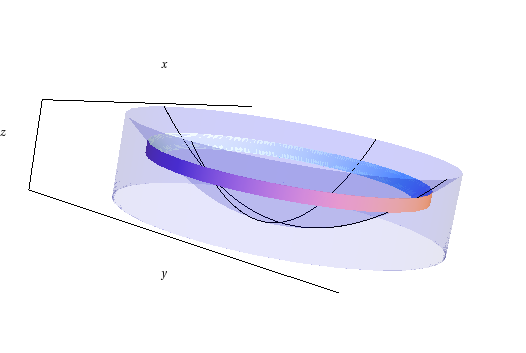
\includegraphics[width=0.5\textwidth]{exam1_s4_4.png}\end{center}
    Then the horizontal component of the normal force, $N_x$, is distributed over an area of
    \begin{equation}
      \Delta z 2 \pi\left(r + \frac{\Delta r}{2}\right).
    \end{equation}
    The vertical component of the normal force, $N_z$, is distributed over an area of
    \begin{equation}
      \pi \left( \left(r + \frac{\Delta r}{2}\right)^2 - \left(r - \frac{\Delta r}{2}\right)^2\right).
    \end{equation}
    Then, approximately equating the pressures, combining the two equations above with \autoref{eq:4:N_x} and \autoref{eq:4:N_y},
    \begin{equation}
      P \approx \frac{\Delta m \frac{v^2}{r \pm \Delta r}}{\Delta z 2 \pi\left(r + \frac{\Delta r}{2}\right)} \approx \frac{\Delta m g}{\pi \left( \left(r + \frac{\Delta r}{2}\right)^2 - \left(r - \frac{\Delta r}{2}\right)^2\right)}.
    \end{equation}
    Substituting in $r \omega = v$ and $\Delta z = \Delta r \tan\theta$ (since $\tan\theta = \frac{\Delta z}{\Delta r}$), expansion and simplification gives
    \begin{equation}
      \cot \theta \approx \frac{g \left(r+\frac{\Delta r}{2}\right) (r\pm \Delta r)}{r^3 \omega^2}.
    \end{equation}
    Taking the limit as $\Delta r \to 0$,
    \begin{equation}
      \cot \theta = \frac{g}{r \omega^2}.
    \end{equation}
    We also have that $\tan\theta$ is the slope of the tangent line:
    $$\frac{r\omega^2}{g} = \tan\theta = \frac{dz}{dr}.$$
    Manipulating the differentials and integrating both sides,
    $$z = \int_0^z\,dz = \int_0^r \frac{r\omega^2}{g}\,dr = \frac{1}{2}\frac{\omega^2}{g}r^2 = \frac{\omega^2 r^2}{2g}.$$

\end{solution}

\end{document}
